\section{Background}
\label{sec:background}


This section presents background information on human detection	and tracking approaches and related techniques as well as the most popular sensing devices. In  particular, it gives a brief description of the Microsoft Kinect for Windows (K4W) sensor.  In addition, we give an overall picture of the methods and counting logic useful to our occupancy counter software.

\subsection{Human Detection and Tracking}
Human detection and tracking (HDT) is an active research subfield of object recognition. Detecting the presence of humans in a particular environment and planing resources accordingly are at the core of many problem-solving strategies in construction management. Human motion tracking includes capturing body displacements and limb movements such as postures and gestures of human targets. These strategies should be able to predict through a learning mechanism, an acceptable number of occupants of a room  \cite{realtimepeoplecount}. Such prediction is important in overcoming the necessary time delay between signal detection and appropriate temperature.

\subsubsection{Approaches in HDT}
HDT is by nature a complex process that includes issues as simple as adequate sensing to the delicate data-mining techniques. It is a challenging task for a number of reasons. The common obstacles to quality detection and tracking are ambient noise, device imperfection, environmental factors variation, fluctuation of data collected, background signal similarity and sometimes, intentional deception (adversarial scenario). Our interest in this study is limited to the well known spatio-temporal properties related to the position and history (tracks) of human present in a given environment. These properties are presence, count, location, track and identity.

\subsubsection{Sensor Technologies for HDT}
Several kinds of counters that require contact with people, such as turnstiles, are used because contact type counters count very accurately. These counters, however, cannot be applied to spaces within commercial buildings because, except at a few critical places (e. g. , entrances), they obstruct the normal flow of people in work spaces and would require installation in each room \cite{Yoshinaga}. Several kinds of sensors currently can provide information on occupancy, such as video cameras equipped with occupancy counting software, optical tripwires and pyroelectric infrared (PIR) motion sensors that count the number of people crossing a particular area. Wireless sensor networks have been widely used as supported technologies for monitoring, tracking and controlling Human Mobility. Most of studies designed a WSN for occupancy detection and result data analysis to send a final control function to the thermostat for HVAC monitoring. The authors of \cite{TinyAgent} highlighted another approach in occupancy detection by using sensors called Tiny Agents (TA) to control power consumption in a building. The tiny agents are distributed throughout the building and deployed in air-conditioning system to capture and send room temperatures and interact with the AC or other agents.

\subsubsection{Occupancy Counters}
An Occupancy Counter is a system that counts the number of persons entering and exiting a room. Many devices based on several technologies (ex. Cameras, infrared beams, vision) have been used with various level of success in commercial systems to count people indoor and outdoor.Remarkable research using 1) neural networks to count subjects in video images and 2) algorithms that use single or multiple lines as counting zones  have also been proposed.

\subsection{The Microsoft Kinect Sensor}
 The Kinect sensor is a motion sensing device with an infrared depth sensor , an emitter and a microphone sound system built around an maleable RGB camera as shown in Figure \ref{fig:kcom}.  Kinect array specification include  a 43 degrees vertical angle viewing  and 57 horizontal degrees  of field of view. This is a motion sensing input that enables a user to remote control a host system via gesture and sound commands. Optical and acoustical detections are the motion sensing that can be electronically identified. Infrared light or laser technology may be used for optical detection because Kinect is an electronic sensor. The Kinect sensor also performs functions such as voice recognition, facial recognition, and skeletal tracking along with motion detection \cite{aboutkinect}. The depth camera, a virtual camera, is the result of displacement matching on the IR projector and real IR camera, each equipped with its own lens distortion.  The depth data from Kinect sensor is the distance, in millimeters, to the nearest object at that particular (x, y) coordinate in the depth sensor’s field of view.

\begin{figure} [!ht]
  \begin{center}
	  	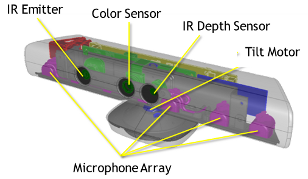
\includegraphics[width=0.9\columnwidth]{./images/k4w350.png}
  \end{center}
  \caption{Kinect component}\label{fig:kcom}
\end{figure}

There are a variety of open source libraries for Kinect programming using PC's like libfreenect, openni and SDK. Open Kinect \cite{openkinect} is community of people who use libfreenect, a free and open source library for enabling Kinect programming in PC’s run by Windows, Linux, and Mac. Open-Kinect support many wrappers like python, c++, c]. The official library from Microsoft Kinect SDK  provides features like color images, depth images, audio input, and skeletal data. The tracking mechanism in software technology used in Kinect enables advanced gesture, facial and voice recognitions.
